\section{Summary}

A selection designed to be uniformly efficient in all regions of the dark boson's mass-lifetime
parameter space has been presented with a view to embarking on a search for a new dark boson.
A frequentist method designed to search for an signal in any arbitrary mass spectrum has also been
presented and used in the case of the dimuon mass spectrum from \btokstrmumu.

This strategy has extracted a $p$-value of a particle considering test masses which do not go all
the way to the boundaries of various vetoes in the invariant dimuon mass spectrum.
It is determined that the maximum deviation of the selected candidates from the null hypothesis of
zero signal has a global significance of $0.48\stdev$ at $m_t = 4285.0\mev$.
This is consistent with no new particle in the \mumu distribution over the mass ranges probed.
The full analysis will get much closer to these edges and probe the interesting $m_{\mumu}=214\mev$
region.
The next step in the analysis is to set limits and present them in a model independent way.
Of course, they can be translated to specific models for interpretation.

%Figure~\ref{fig:db:excl} shows projected exclusion regions from this analysis.
%Figure~\ref{fig:db:excl:inf} shows projected exclusion regions for the inflaton
%model~\cite{Bezrukov:2014nza}, and axion model~\cite{Freytsis:2009ct}.

Figure~\ref{fig:db:excl:infl} shows the projected
sensitivity of this analysis to the inflaton model in Ref.~\cite{Bezrukov:2014nza}.
There is a region excluded by theory, where the model does not satisfy known cosmological
constraints.
It is predicted that it should be possible to rule out the mass range
$250<\mass{\db}<450\mev$ entirely, and come within an order of magnitude of mixing parameter
$\theta^2$ for masses up to $1000\mev$.
Assumptions made in making this are that: the lifetime of the inflaton is in the range
$1<\lifetime{\db}<1000\ps$, that $\BF(\btokstrdb)\simeq10^{-6}$,
and that the \db has the same couplings as the Higgs boson.
%and that $\BF(\dbtomumu)$
%is the same for a Higgs boson with the mass of an inflaton.

\begin{figure}
  \begin{center}
    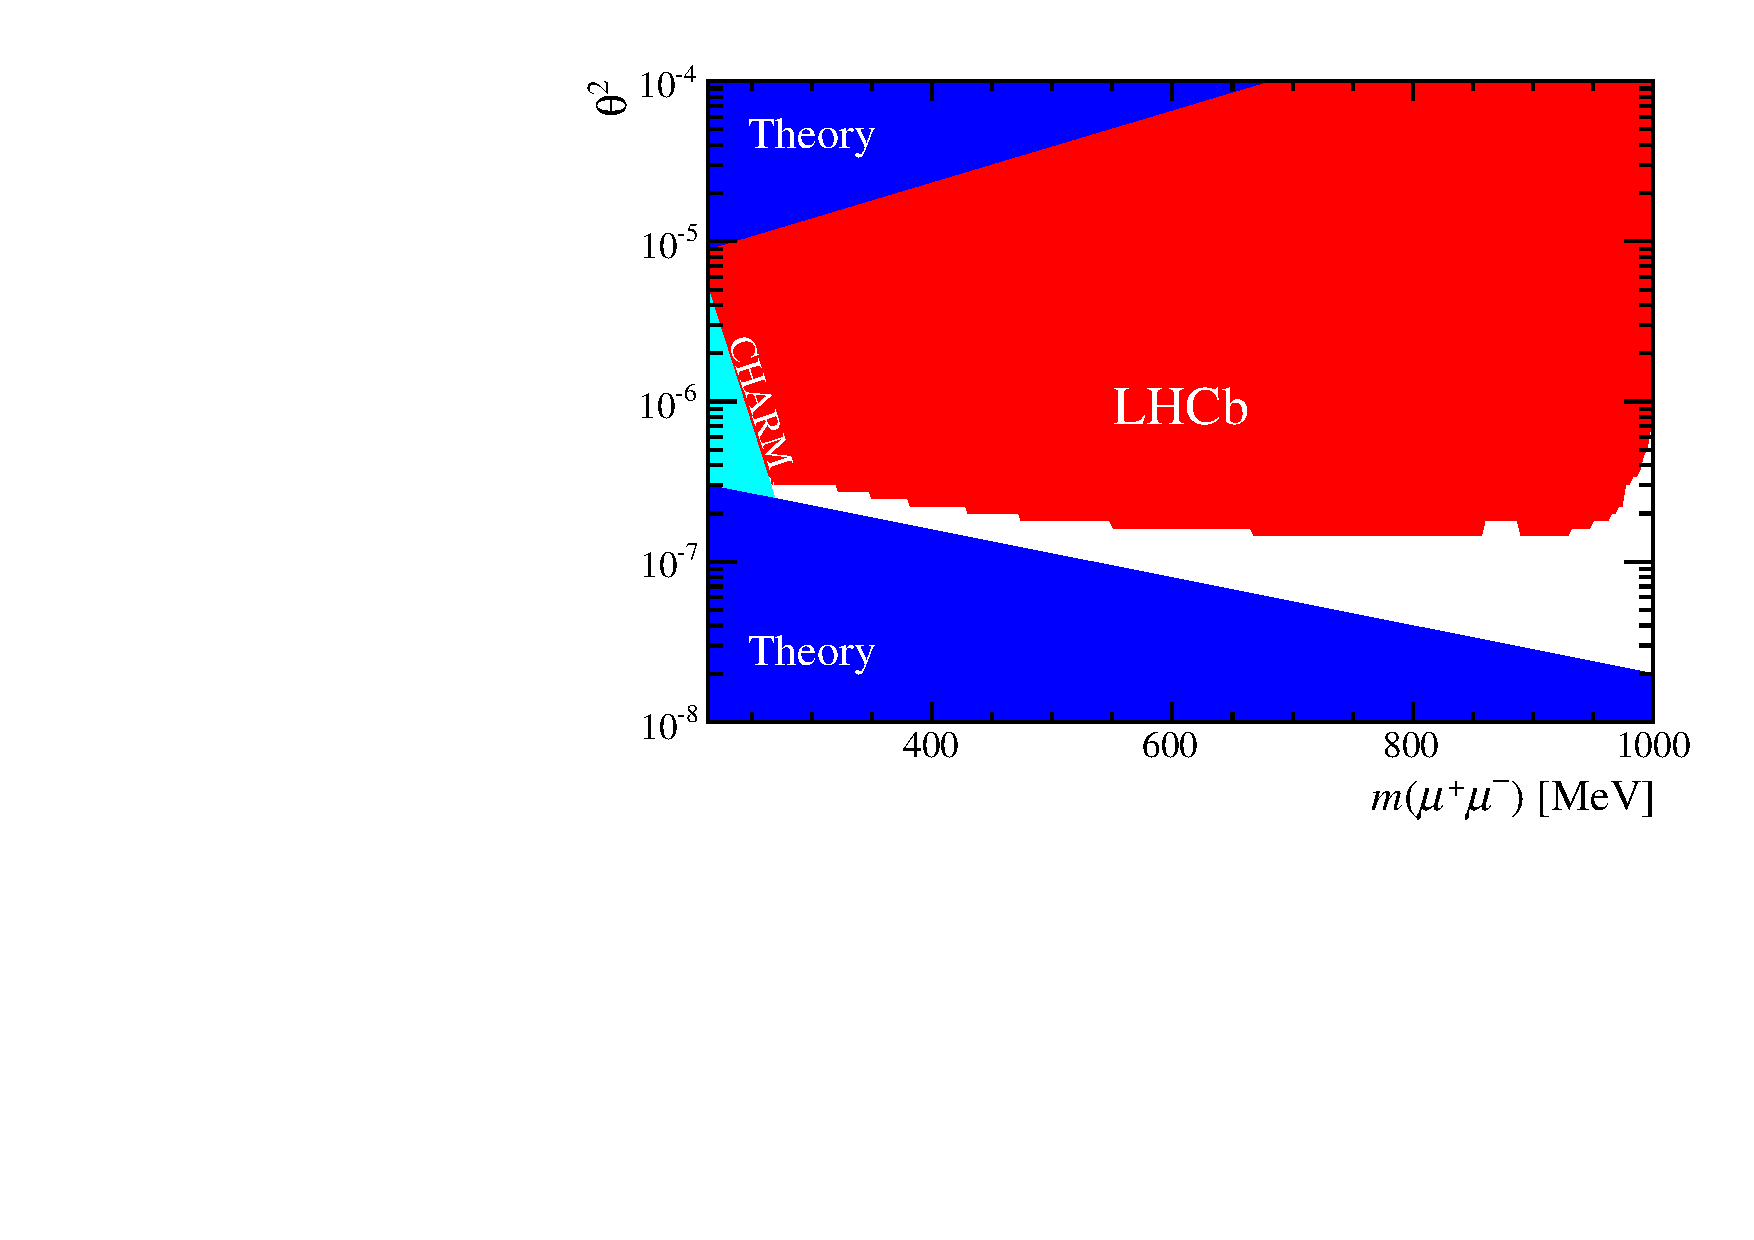
\includegraphics[width=0.65\textwidth]{kstmm_infl_excl}
    \caption[Projected sensitivity in an inflaton search]
    {
      Projected exclusions for an inflaton model from Ref.~\protect\cite{Bezrukov:2014nza}, in the
      mass range $1<\mass{\db}<1000\mev$.
      The region below the red line is excluded by theory, since the model fails cosmological
      constraints in this region.
      In this mass range, it is expected that this analysis will exclude all but a small area of
      parameter space for this model.
    }
    \label{fig:db:excl:infl}
  \end{center}
\end{figure}






